\chapter{Resultados y discusión}

\section{Análisis e interpretación de la información}


\subsection{Proceso de clasificación, registro y codificación de los datos}


En el presente estudio se utiliza datos que corresponden a  planes de estudio de algunas universidades del país y de modelos de planes de estudio que representan una implementación de guías internacionales. 

Esa decisión se da ante la premisa que el contenido de un curso aborda las áreas de conocimiento esperado de un programa de estudios en informática. Por ejemplo, un curso de sistemas operativos (SO) se presume comparable entre distintas propuestas universitarias y ejemplos de guía internacional. 

Esa es una primera aproximación que no debe ser descartada aún si los enfoques o niveles de alcance de cada curso sean distintos, algo que se podrá analizar a futuro,  cuando se compare el contenido de áreas de conocimiento de cada curso y los respectivos ejemplos de cursos de las guías. 

Con esa premisa o función comparable podremos realizar una codificación con un mismo $(ID,NOMBRE)$ que nos permita hacerlos identificables entre los planes de estudio y guías. De esa manera podremos encontrar relaciones a nivel de grafos.

A continuación utilizamos solo unas muestras de planes y guías para mostrar el proceso de codificación. El detalle se encuentra en el enlace del anexo \ref{ane:anexo1} que aparecerá en el anexo del documento.

\begin{table}[H]
\centering
\caption{Guia ACM 68}
\begin{tabular}[t]{lccl}
\hline
Id&Nombre&Relacion&NombreCurso\\
\hline
1&B1&-&Introduction to Computing\\
2&M1&-&Introduction to Calculus\\
3&B2&(3,1)&Computer and Programming\\
4&M3&(4,2)&Linear Algebra\\
5&M2&(5,2)&Mathematical Analysis I\\
6&B3&(6,1),(6,5),(6,4)&Introduction to Discrete Structures\\
7&B4&(7,4)&Numerical calculus\\
8&M2p&(8,2)&Probability\\
9&M4&(9,5),(9,4)&Mathematical Analysis II\\
10&I1&(10,5),(10,6)&Data Structures\\
11&I2&(11,3),(11,6)&Programming Languages\\
12&I3&(12,3)&Computer Organization\\
13&M7&(13,8)&Probabilty and Statistic\\
29&M6&-&Algebraic Structures\\
14&M5&(14,8)&Advance Multivariable Calculus\\
15&I4&(15,10),(15,11)&Systems Programming\\
30&I5&(30,10)(30,11)&Compiler Construction\\
16&I6&(16,12) (16,6)&Switching Theory\\
17&I7&(17,6)&Sequential Machine\\
25&I8&(25,9)&Numerical Analysis I\\
26&I9&(26,9)&Numerical Analysis II\\
18&A1&(18,10)(18,11)&Formal Languages and Syntactic Analysis\\
27&A2&(27, 12)&Advance Computer Organization\\
28&A3&(28, 6), (28, 11)&Analog and Hybrid Computing\\
19&A4&(19,14)(19,13)&System Simulation\\
20&A5&(20,9)&Information Organization and Retrieval\\
21&A6&(21,9)&Computer Graphics\\
22&A7&(22,6) (22,17)&Theory of computability\\
23&A8&(23,19)&Large Scale Information Processing System\\
24&A9&(24,9)&Artificial Inteligence and Heuristic programming\\
\hline
\end{tabular}
\label{tab:tabacm68}
\end{table}

\begin{table}[H]
\centering
\caption{Guia ACM 2001}
\begin{tabular}[t]{lccl}
\hline
Id&Nombre&Relacion&NombreCurso\\
\hline
1&cs101		&-		&Programming Fundamentals\\
2&cal1		&-		&Calculus I\\
3&cs102I	&(3,1)	&The Object-Oriented Paradigm\\
4&cs115		&(4,2)	&Discrete Structures for Computer Science\\
5&cal2		&(5,2)	&Calculus II\\
6&sc120		&-		&Science course I\\
7&cs103i	&(7,3)	&Data Structures and Algorithms\\
8&cs210		&-		&Introduction to Computer Organization\\
9&sc		&-		&Science Course II\\
10&ps		&(10,5)	&Probability and Statistics\\
11&cs210	&(11,4)	&Algorithm Design and Analysis\\
12&cs220	&(12,3	&Computer Architecture\\
13&am		&(13,5)	&Advanced Mathematics elective\\
14&cs225	&(14,12)&Operating Systems\\
15&cs280	&-		&Social and Professional Issues\\
16&cs230	&(16,14)&Net-Centric Computing\\
17&cs262	&-		&Information and Knowledge Management\\
18&cs290	&(18,4)	&Software Development\\
19&cs115	&-		&Discrete Structures for Computer Science\\
20&cn1(e)	&(20,2)	&Numerical analysis\\
21&cs302(a)	&(21,10)&Probability and Statistics\\
22&cs270T	&(22,4)	&Databases\\
23&CS307(a)	&-		&Simulation and Modeling\\
24&CS340	&-		&Compiler Construction\\
25&GV11(e)	&-		&Computer vision\\
26&CS306	&-		&Operations Research\\
27&cs222	&(27,12)&Architectures for Networking and Communication\\
28&cs250	&(28,3)	&Human-Computer Interaction\\
29&cs260	&(29,4)	&Artificial Intelligence\\
30&IM10(e)	&-		&Data mining\\
\hline
\end{tabular}
\label{tab:tabsacm2001}
\end{table}

\begin{table}[!ht]
\centering
\caption{Guia ACM 2013}
\begin{tabular}[t]{lcccl}
\hline
Id&KA&Nombre&Relacion&NombreCurso\\
\hline
1&-	&MAT171&-&Calculus I\\
2&-	&CSC221&-&Introduction to Programming\\
3&AL&CSC207&(3,2)&Object-Oriented Programming\\
4&AR&CS552&(4,2)&Intro to Computer Architecture\\
5&AR&COSCMat201&(5,1)&Modeling and Simulation\\
6&CN&CS175&-&Computer Graphics\\
7&DS&MAT267&(5,1)&Discrete Mathematics\\
8&AL&CSC140&(8,7)&Algorithms\\
9&IAS&CS475&(9,3)&Computer Systems Security\\
10&IM&CSU-DS&(10,4)&Database Systems\\
11&IS&UH-AI&(11,7)&Artificial Intelligence\\
12&NC&CWRU&(12,4)&Computer Networks I\\
13&OS&RU STY1&(13,4)&Operating Systems\\
14&PD&NNSU-IPP&(14,13)&Introduction to Parallel Programming\\
15&PL&Utrect-LC&(15,2)&Languages and Compilers\\
16&PL&215&(16,2)&Software Development Foundations\\
17&HCI&FIT3063&(17,16)&Human Computer Interaction\\
18&SE&CS169&(18,8)&Software Engineering\\
19&SF&CS2200&(19,12)&Computer Systems and Networks\\
20&SP&CMU-TEGS&-&Technology, Ethics, and Global Society\\
21&AL&CSC301&(21,8)&Analysis of Algorithms\\
22&PBD&CSWP&(22,3)&Web Platforms\\
23&PBD&CSMP&(24,3)&Mobile Platforms\\
24&AL&CSCI136&-&Data Structures and Advanced Programming\\
\hline
\end{tabular}
\label{tab:tabsacm2013}
\end{table}

\newpage

En  \ref{tab:tabacm68} tenemos un ejemplo de plan de estudio y sus relaciones de un plan de estudios de la enseñanza de la informática, modelo conocido como el primer intento de ordenar el programa de estudios de la informática (ACM68). La difusión de ese estándar o modelo no tenía el impacto que permite en la actualidad la difusión de innovaciones o modelos internacionales, pero de alguna manera influenció el desarrollo de las propuestas educativas que han existido en el país. En \ref{tab:tabsacm2001} y \ref{tab:tabsacm2013} tenemos ejemplos de cursos modelos y sus relaciones según los referentes ACM2001 y ACM2013. 

\begin{table}[H]
\centering
\caption{Sistemas 2009 con Acm68}
\begin{tabular}[t]{|llllll|}
\hline
Id & Nombre & Relacion &  IdUnificado & model1 & model2 \\
\hline
1 & ma1 & - & 2 & - & - \\
2 & cal1 & -  & 5 & - & - \\
3 & algo1 & - & 3 & - & - \\
4 & intro1 &- & 1 & - & - \\
6 & algo2 & (6,3)  & 11 & (11,3),(11,8) & (11,3) \\
7 & cal2 & (7,2) & 9 & (9,5),(9,4) & (9,5) \\
8 & mat2 & (8,1) & 4 & (4,2) & (4,2) \\
10 & estruc1 & (10,3)  & 10 & (10,3),(10,6) & (10,3) \\
11 & algo3 & (11,8) &  22 & (22,6),(22, 17) & (22,10) \\
12 & matd & (12,7)  & 6 & (6,1) & (6,4) \\
13 & e1 & (13,6) & 8 &	(8,2) & (8,9) \\
15 & comg & (15,9) & 21 & (21,10) & (21,30) \\
17 & ed & (17,6) &	- &(14,9) & (14,9) \\
18 & cd & (18,16) & - &	(16,6),(16, 12) & (16,44) \\
19 & e2 & (19,13) & 13 &(13,8) & (13,8) \\
20 & bd1 & (20,22) & 20 & (20,10) & (20,45) \\
21 & mn & (21,13) & 7 & (7,1),(7,5),(7,4) & (7,14) \\
22 & lg & (22,9),(22,10)  & 18 & (18,10)(18,11) & (18,22)(18,6) \\
23 & dg & (23,14) & 17 &(17,6),(17, 16)&(17,16) \\
26 & arq & (26,19) & 12 & (12,3),(12,8) & (12,17) \\
27 & so & (27,18)  & 15 & (15,10),(15,11),(15,12) & (15,18)	\\
32 & ia & -  & 24 & (24,10) & (24,34) \\
33 & mo & -  & 19 & (19,15),(19,13) & (19,29) \\
34 & net & -  & 23 & (23,19) & (24,12)(24,15) \\
37 & sd & - & 25 & (25,12) & (25,23) \\
\hline
\end{tabular}
\label{tab:tabsis2009}
\end{table}

\newpage

\begin{table}[H]
\centering
\caption{Sistemas 2017}
\begin{tabular}[t]{lccc}
\hline
Id&Nombre&Relacion&NombreCurso\\
1&ca1&calculo I&-\\	
2&aal&algebra y geometria analítica	&-\\
3&cal2&calculo II&-\\	
4&fis1&fisica I&-\\	
5&q1&quimica general&-\\	
6&cal3&calculo III&-\\	
7&pa1&Programación y fundamentos de algoritmica&-\\	
8&ts&Teoría general de sistemas&-\\	
9&e2&Estadistica&-\\	
10&sed&Series y ecuaciones diferenciales				&(10,6)\\
11&md&Matemáticas Discretas	&-\\
12&apo&Algoritmica y programación orientada a objetos	&(12,7)\\
13&mn&Metodos numéricos									&(13,9)\\
14&pm&Probabilidades y muestreo							&(14,9)(14,10)\\
15&fis&Fisica electrónica y sistemas digitales			&(15,10)\\
16&bd&Base de Datos										&(16,12)\\
17&daa&Diseño y Análisis de Algoritmos					&(17,12)\\
18&edd&Estructura de datos								&(18,12)\\
19&asi&Analisis de Sistemas de Información	&-\\
20&ms&Modelos y Simulación								&(20,13)(20,14)\\
21&aq&Arquitectura de Computadoras						&(21,15)\\
22&lc&Lenguajes y Compiladores							&(22,11)\\
23&bid&Big Data											&(23,16)(223,17)\\
24&cv&Computación Visual	&-\\
25&ds&Diseño de Sistemas de Información					&(25,19)\\
26&io&Investigación Operativa							&(26,20)\\
27&rta&Redes Transmisión y Automatización y Control		&(27,21)\\
28&so&Sistemas Operativos	&-\\
29&ih&Interacción hombre computador						&(29,24)\\
30&in&Inteligencia de Negocios	&-\\
31&dsw&Desarrollo de Sistemas Web						&(31,25)(31,23)\\
32&fwp&Formulación y Evaluación de Proyectos			&(32,26)(32,25)\\
33&ia&Inteligencia Artificial							&(33,26)(33,22)\\
\hline
\end{tabular}
\label{tab:tabsis2017}
\end{table}


\newpage

En  \ref{tab:tabsis2009} y \ref{tab:tabsis2017} tenemos una lista de cursos del programa de estudios de ingeniería de sistemas 2009 y 2017 respectivamente, con una columna que identifica el curso equivalente del modelo de ACM 68 en el primer caso y se hace lo mismo con los programas o referentes que queremos realizar la comparación, por motivos de espacio no incluiremos todas las tablas aquí, pero se incluyen como enlaces en el anexo del documento.

El proceso de modelamiento de la información de las curriculas pasa por establecer un $(ID,Nombre)$ que servirá para las comparaciones así como establecer dos modelos de grafos que usaremos para la comparación. Establecemos los siguientes pasos para el modelamiento:

\begin{enumerate}
	\item Usamos una tabla de $(ID,Nombre)$ para cada guía o plan que queremos comparar.

	\item Para realizar las comparaciones, establecemos un indice común que nos permita realizar la selección de elementos comunes.

	\item Establecemos como $Modelo_1$ a la comparación que incluye los nodos y relaciones del grafo $G_1$ y se identifica la existencia de los mismos nodos y relaciones con el grafo $G_2$. La codificación de las relaciones considera las dependencias del grafo $G_1$

	\item Establecemos como $Modelo_2$ a la comparación que incluye los nodos y relaciones del grafo $G_1$ y se identifica la existencia de los mismos nodos y relaciones con el grafo $G_2$. La codificación de las relaciones considera las dependencias del grafo $G_1$ y $G_2$ respectivamente. Es decir se comparan cada grafo considerando sus relaciones originales.

\end{enumerate}

Para la comparación a nivel de cursos si requiere inferir para la codificación el alcance de las posibles unidades de conocimiento identificados en los planes de estudio de las universidades que estamos analizando. Dado el alcance en tiempo y revisión, solo mostraremos comparaciones de pocos cursos pero sentando las bases de la factibilidad según las hipótesis de la presente investigación.
%ToDO Codificación de comparación de cursos



\subsection{Técnica analítica}

Para el análisis de identificación de relaciones usaremos la teoría de grafos modelando los planes, guías internacionales y cursos siguiendo una representación de grafos. Posteriormente usaremos propiedades de la teoría de grafos para encontrar similaridad, distancias, sub-grafos comunes y valores cuantitativos que indiquen la cantidad de relaciones comunes entre ambos modelos a comparar. Como se explica en \ref{TeoriaGrafo} usaremos el modelamiento de grafos y los algoritmos respectivos para identificar similaridad y valore cuantitativos.

Nuestra hipótesis central es la siguiente:

\begin{enumerate}

	\item P1. (H1) Dado un modelo en grafos de un plan de estudios o una guía internacional encontrar la relación entre un plan de estudios $G_1$ y $G_2$ como la métrica entre ambos modelos usando el concepto de similaridad grafos. De modo que la similaridad es significativa. 

\end{enumerate}

Dada la métrica que consideramos en el estudio:

\begin{center}

 $\delta(g,g^\prime)=1-\frac{|mcs(g,g^\prime)|}{max(|g|,|g^\prime|)}$

\end{center}

Que a su vez depende de encontrar el Máximo común sub-grafo $MCS$ que en el presente estudio depende de un algoritmo indicado en \ref{Algoritmo}. Con los datos indicados previamente modelaremos planes, guías internacionales cursos como grafos y encontraremos la métrica para validar las respectivas hipótesis propuestas.

Las hipótesis secundarias se enumeran a continuación:

\begin{enumerate}


	\item P2. (H2)	Dado un grafo $G_1$ que representa una profesión de ingeniería de sistemas o informática y $G_2$ un referente internacional de ACM/IEEE u otro. Identificar que la similaridad es significativa. 

	\item P3. (H3) Dado un grafo $G_1$ que representa el plan de estudio de una carrera vinculada a la informática de un año $X$ y $G_2$ un plan de la misma carrera pero del año $Y$. Identificar que la similaridad es significativa.


\end{enumerate}

	Como se indico en el capitulo 3 tendremos 2 métricas para evaluar nuestras hipótesis. 

	El nivel de similaridad entre 2 grafos como el valor $ z = 0.2 $ como el valor que indique o no la presencia significativa de similaridad. Un valor mayor a $z$ refleja un nivel aceptable de similaridad, un valor menor indica que no existe similaridad.

	Otro elemento que podemos considerar es la proporción en una de los planes o guías respecto a la cantidad de nodos en común. En este caso usaremos una proporción $ t = 0.1$ para indicar cierto grado de similaridad por nodos. Esto significa que un valor menor a $t$ significa que no existe similaridad en cantidad de nodos en común.

\section{Pruebas de hipótesis}


Tal como planteamos en el capitulo anterior de metodología, se sigue una serie de pasos para codificar los datos en grafos. En la siguiente tabla se muestra los datos recolectados de los planes y guías consideradas para el experimento.



\begin{table}[H]
\centering
\caption{Tabulación de datos sobre comparaciones}
\begin{tabular}[t]{|l|l|l|l|l|l|}
\hline
Caso & Modelo & G(acm68)-n & G(acm68)-e & H(sis2009)-n & H(sis2009)-e\\
1&model1&30&39&41&34\\
\hline
1&model2&30&39&42&32\\
\hline
Caso & Modelo & G(acm68)-n & G(acm68)-e & H(sis2017)-n & H(sis2017)-e\\
2&model1&30&39&38&25\\
\hline
2&model2&30&39&38&24\\
\hline
Caso & Modelo & G(sis2009)-n & G(sis2009)-e & H(sis2017)-n & H(sis2017)-e\\
3&model1&30&39&38&25\\
\hline
3&model2&30&39&38&24\\
\hline
Caso & Modelo & G(acm2013)-n & G(acm2013)-e & H(sis2017)-n & H(sis2017)-e\\
4&model1&30&39&38&25\\
\hline
4&model2&30&39&38&24\\
\hline
Caso & Modelo & G(acm2013)-n & G(acm2013)-e & H(pucp2020)-n & H(pucp2020)-e\\
5&model1&26&20&60&20\\
\hline
5&model2&26&20&60&17\\
\hline
Caso & Modelo & G(acm68)-n & G(acm68)-e & H(unisis2018)-n & H(unisis2018)-e\\
6&model1&30&39&27&15\\
\hline
6&model2&30&39&27&18\\
\hline
\end{tabular}
\label{tab:tabcomparaciones}
\end{table}


\clearpage

\section{Presentación de Resultados}

Presentaremos ahora los resultados organizados por casos. Es importante explicar algunas caracteristicas de las visualizaciónes:

\begin{enumerate}
	\item Por cada caso se dan dos comparaciones, denominadas $Modelo_1$ y $Modelo_2$.
	\item El $Modelo_1$ representa la comparación de los nodos y enlaces del grafo $G_1$ y la busquedad de similitud en el grafo $G_2$. Las relaciones se consideran priorizando las relaciones del grafo $G_1$
	\item El $Modelo_2$ representa la comparación de los nodos y enlaces del grafo $G_1$ y la busquedad de similitud en el grafo $G_2$. Las relaciones se consideran respetando las relaciones del grafo $G_1$ y las relaciones del grafo $G_2$ respectivamente.
	\item Los enlaces comunes a ambos grafos aparecen en color naranja.
	\item Los enlaces aparecen en color azul.
	\item Los nodos del modelo en amarillo.
	\item Los nodos del MCS en color verde

\end{enumerate}

\subsection{Caso 1 Hipotesis Secundaria 1}

A continuación se muestran las representaciones gráficas y los resultados del $Caso_1$ de la comparación entre un plan de estudio: Sistemas 2009 y la guía internacional ACM 68. Como podemos observar en la figura \ref{fig:modelo1} y la figura \ref{fig:modelo2} se muestra la identificación de un maximo común sub-grafo. En el primer ejemplo se muestra la comparación de un modelo de curricula de ingeniería de sistema del 2009 codificado y comparado con un modelo clásico de curricula de computación de acm68. Como se ha indicado previamente la codificación de las relaciones fuerza de alguna manera a la existencia de un sub-grafo teniendo en cuenta que el modelo 1 representa la identificación de nodos comunes y toma los enlaces considerando las relaciones del modelo G en este caso del ACM 68. En en el caso del modelo 2 se respetan las relaciones del 

\begin{figure}[H]
\centering
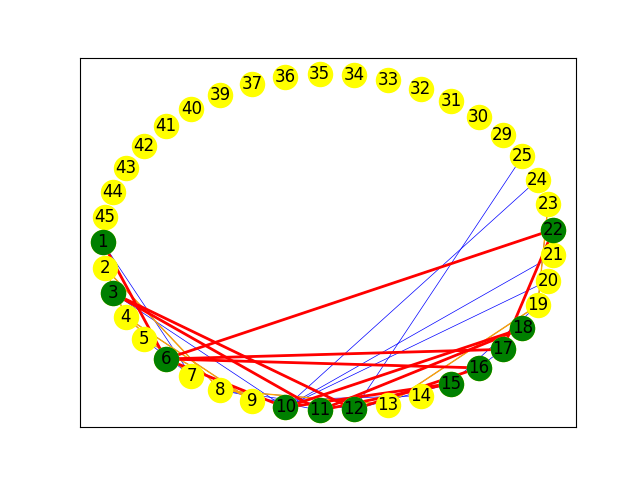
\includegraphics[width=0.7\linewidth]{images/sis2009/H_sis2009_cmp_acm68_m1_mcs_mix}
\caption{Sis2009 ACM68 MCS modelo 1}
\label{fig:modelo1}


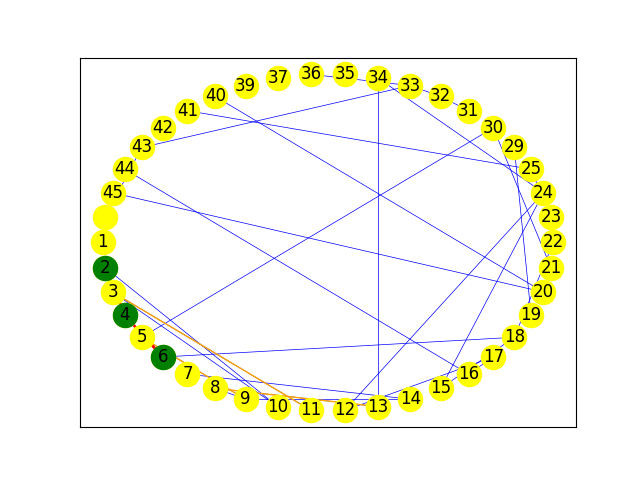
\includegraphics[width=0.7\linewidth]{images/sis2009/H_sis2009_cmp_acm68_m2_mcs_mix}
\caption{Sis2009 ACM68 MCS modelo 2}
\label{fig:modelo2}

\end{figure}

\begin{table}[H]
\centering
\caption{Tabulación de datos sobre comparaciones}
\begin{tabular}[t]{|l|l|l|l|l|l|}
\hline
Caso & Modelo & G(acm68)-n & G(acm68)-e & H(sis2009)-n & H(sis2009)-e\\
1&model1&30&39&41&34\\
\hline
1&model2&30&39&42&32\\
\hline
\end{tabular}
\label{tab:tabcomparaciones_P2}
\end{table}


\begin{table}[H]
\centering
\caption{Comparación G-ACM 68 y H-Sistemas 2009}
\begin{tabular}[t]{lccccc}
\hline
Caso & Modelo & MCSsubgrado & similaridad & nodos & enlaces \\
1 & $modelo_1 $ & 0.64285714 & $z=0.35714286$ & 11 & 13\\
1 & $modelo_2 $& 0.9285714286 & $z=0.07142857143$ & 3 & 2\\
\hline

\end{tabular}
\label{tab:tabcomparaciones_P2}
\end{table}

\begin{table}[H]
\centering
\caption{Tabla de resultados de proporcionalidad}
\begin{tabular}[t]{lccccccccc}
\hline
Caso & Modelo & nodosCom & enlacesCom & proporcionG &proporcionH \\
1 & $modelo_1$ & 20 & 21 & $t_1=0.6666666667$ & $t_2=0.487804878$ \\
1 & $modelo_2$ & 9 & 5 & $t_1=0.3 $ & $t_2=0.2142857143$ \\
\hline
\end{tabular}
\label{tab:tabresultados2_P2}
\end{table}

\begin{table}[H]
\centering
\caption{Tabla de Hipotesis vs Resultados }
\begin{tabular}[t]{lccccc}
\hline
Hipotesis & Caso & modelo & Similaridad & ProporcionG & ProporcionH\\
P2 & 1 & modelo1 & $z>0.2$ & $t_1>0.1$ & $t_2>0.1$ \\
P2 & 1 &modelo2 & $z<0.1$ & $t_1>0.1$ & $t_2<0.1$\\
\hline
\end{tabular}
\label{tab:hipotesis_P2}
\end{table}

\clearpage

\subsection{Caso 2 Hipotesis Secundaria 1}

A continuación se muestran las representaciones gráficas y los resultados del $Caso_2$ de la comparación entre un plan de estudio: Sistemas 2017 y la guía internacional ACM 68. Las comparaciones muestran en la figura \ref{fig:c2p2modelo1} la comparación asumiendo que los nodos respetan la red de relaciones de acm68 y en la figura \ref{fig:c2p2modelo2} se muestra el grafo considerando las relaciones 

\begin{figure}[H]
\centering
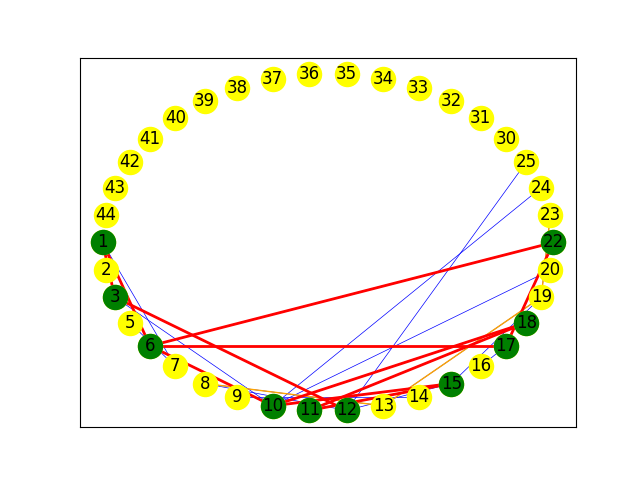
\includegraphics[width=0.7\linewidth]{images/sis2018/H_sis2018_acm68_m1_mcs_mix}
\caption{Sis2017 ACM68 MCS modelo 1}
\label{fig:c2p2modelo1}


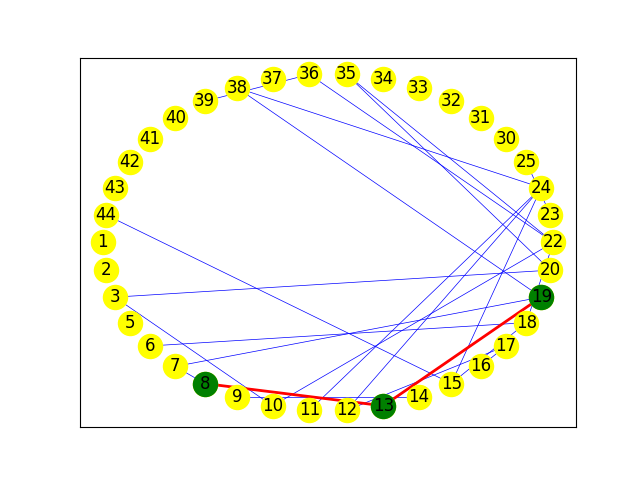
\includegraphics[width=0.7\linewidth]{images/sis2018/H_sis2018_acm68_m2_mcs_mix}
\caption{Sis2017 ACM68 MCS modelo 2}
\label{fig:c2p2modelo2}

\end{figure}


\begin{table}[H]
\centering
\caption{Tabulación de datos sobre comparaciones}
\begin{tabular}[t]{|l|l|l|l|l|l|}
\hline
Caso & Modelo & G(acm68)-n & G(acm68)-e & H(sis2009)-n & H(sis2009)-e\\
2&model1&30&39&38&25\\
\hline
2&model2&30&39&38&24\\
\hline
\end{tabular}
\label{tab:tabcomparaciones_C2_P2}
\end{table}


\begin{table}[H]
\centering
\caption{Comparación G-ACM 68 y H-Sistemas 2009}
\begin{tabular}[t]{lccccc}
\hline
Caso & Modelo & MCSsubgrado & similaridad & nodos & enlaces \\
2 & $modelo_1$ & 0.736842105263158 & $z=0.2631578947$ & 10 & 11\\
2 & $modelo_2$ & 0.9210526316 & $z=0.07894736842$ & 3 & 2\\
\hline
\end{tabular}
\label{tab:tabcomparaciones_C2_P2}
\end{table}

\begin{table}[H]
\centering
\caption{Tabla de resultados de proporcionalidad}
\begin{tabular}[t]{lccccccccc}
\hline
Caso & Modelo & nodosCom & enlacesCom & proporcionG &proporcionH \\
2 & $modelo_1$ & 14 & 14 & $t_1=0.4666666667$ & $t_2=0.3684210526$ \\
2 & $modelo_2$ & 3 & 2 & $t_1=0.1 $ & $t_2=0.07894736842$ \\
\hline
\end{tabular}
\label{tab:tabresultados2_C2_P2}
\end{table}

\begin{table}[H]
\centering
\caption{Tabla de Hipotesis vs Resultados }
\begin{tabular}[t]{lccccc}
\hline
Hipotesis & Caso & modelo & Similaridad & ProporcionG & ProporcionH\\
P2 & 2 & modelo1 & $z>0.2$ & $t_1>0.1$ & $t_2>0.1$\\
P2 & 2 & modelo1 & $z<0.2$ & $t_1>0.1$ & $t_2>0.1$\\
\hline
\end{tabular}
\label{tab:hipotesis_C2_P2}
\end{table}

\clearpage

\subsection{Caso 3 Hipotesis Secundaria 2}

A continuación se muestran las representaciones gráficas y los resultados del $Caso_3$ de la comparación entre un plan de estudio:  Ingeniería de Sistemas 2009 e Ingeniería de Sistemas 2017. Este caso se representa en la figura \ref{fig:c3p3modelo1} y en la figura \ref{fig:c3p3modelo2}. En la primera imagen se muestra una identificación del valor de similaridad teniendo como base al modelo de grafos del plan 2009. 

\begin{figure}[H]
\centering
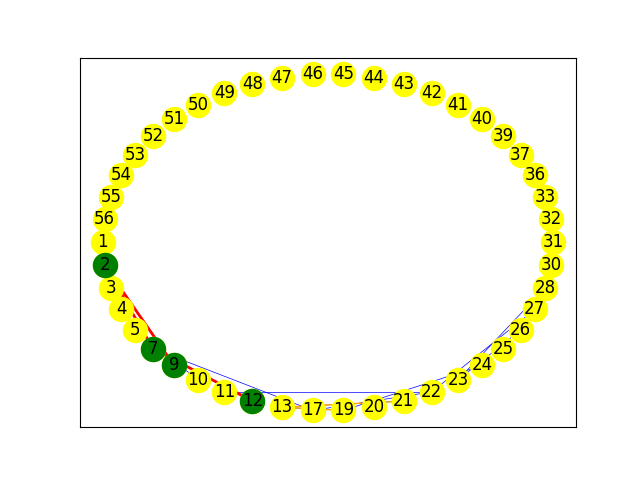
\includegraphics[width=0.7\linewidth]{images/sis2018/H_sis2018_cmp_sis2009_m1_mcs_mix}
\caption{Sis2009 Sis2017 MCS modelo 1}
\label{fig:c3p3modelo1}

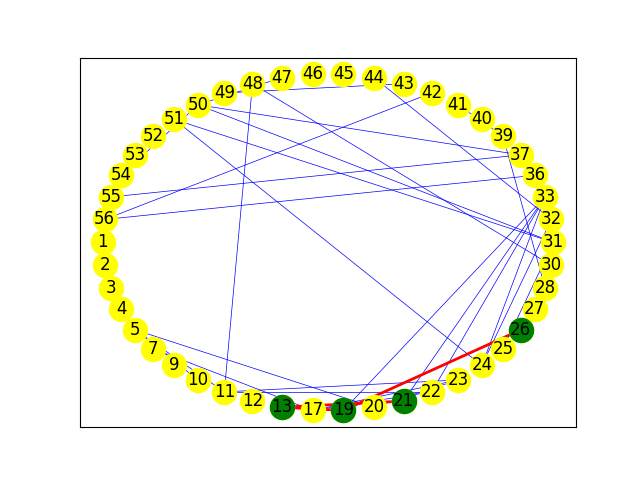
\includegraphics[width=0.7\linewidth]{images/sis2018/H_sis2018_cmp_sis2009_m2_mcs_mix}
\caption{Sis2009 Sis2017 MCS modelo 2}
\label{fig:c3p3modelo2}

\end{figure}


\begin{table}[H]
\centering
\caption{Tabulación de datos sobre comparaciones}
\begin{tabular}[t]{|l|l|l|l|l|l|}
3&model1&30&39&38&25\\
\hline
3&model2&30&39&38&24\\
\hline
\end{tabular}
\label{tab:tabcomparaciones_C_3_P3}
\end{table}


\begin{table}[H]
\centering
\caption{MCS}
\begin{tabular}[t]{lccccc}
\hline
Caso & Modelo & MCSsubgrado & similaridad & nodos & enlaces \\
3 & $modelo_1$ & 0.914893617 & $z=0.08510638298$ & 4 & 3 \\
3 & $modelo_2$ & 0.914893617 & $z=0.08510638298$ & 4 & 3 \\
\hline
\end{tabular}
\label{tab:tabcomparaciones_C_3_P3}
\end{table}

\begin{table}[H]
\centering
\caption{Tabla de resultados de proporcionalidad}
\begin{tabular}[t]{lccccccccc}
\hline
Caso & Modelo & nodosCom & enlacesCom & proporcionG &proporcionH \\
3 & $modelo_1$ & 7 & 5 & $t_1=0.1489361702$ & $t_2=0.152173913$\\
3 & $modelo_2$ & 4 & 3 & $t_1=0.08510638298$ & $t_2=0.08695652174$\\
\hline
\end{tabular}
\label{tab:tabresultados2_C_3_P3}
\end{table}

\begin{table}[H]
\centering
\caption{Tabla de Hipotesis vs Resultados }
\begin{tabular}[t]{lccccc}
\hline
Hipotesis & Caso & modelo & Similaridad & ProporcionG & ProporcionH\\
P3 & 3 & modelo1 &$z<0.2$&$t_1>0.1$&$t_2>0.1$\\
P3 & 3 & modelo1 &$z<0.2$&$t_1<0.1$&$t_2<0.1$\\
\hline
\end{tabular}
\label{tab:hipotesis_C_3_P3}
\end{table}


\clearpage

\subsection{Caso 4 Hipotesis Secundaria 2}

A continuación se muestran las representaciones gráficas y los resultados del $Caso_4$ de la comparación entre un plan de estudio: Ingeniería de sistemas 2017 y ACM 2013. En la figura \ref{fig:c4p2modelo1} se representa la comparación entre grafos priorizando los enlaces de ACM 2013 y en la figura \ref{fig:c4p2modelo2} cada grafo mantiene sus relaciones. 

\begin{figure}[H]
\centering
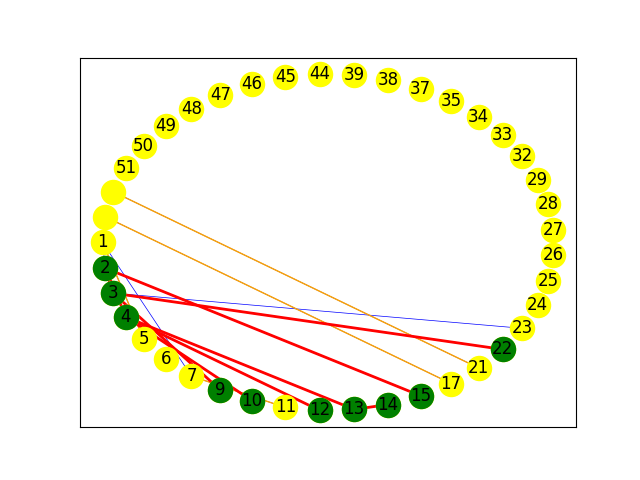
\includegraphics[width=0.7\linewidth]{images/sis2018/H_sis2018_cmp_acm2013_m1_mcs_mix}
\caption{Sis2017 y ACM 2013 MCS modelo 1}
\label{fig:c4p2modelo1}


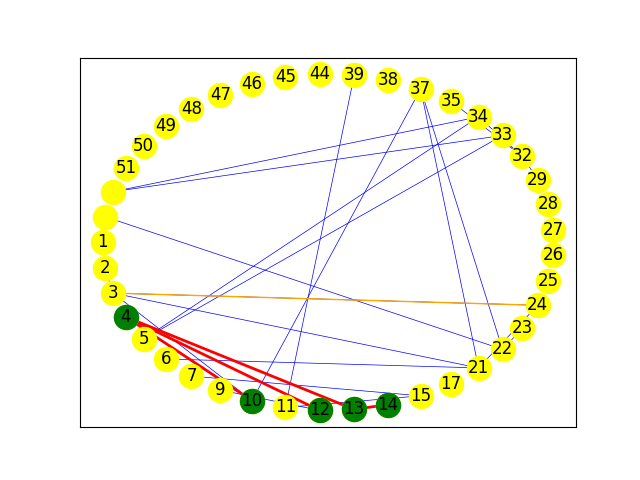
\includegraphics[width=0.7\linewidth]{images/sis2018/H_sis2018_cmp_acm2013_m2_mcs_mix}
\caption{Sis2017 y ACM 2013 MCS modelo 2}
\label{fig:c4p2modelo2}

\end{figure}


\begin{table}[H]
\centering
\caption{Tabulación de datos sobre comparaciones}
\begin{tabular}[t]{|l|l|l|l|l|l|}
\hline
4&model1&30&39&38&25\\
\hline
4&model2&30&39&38&24\\
\hline
\end{tabular}
\label{tab:tabcomparaciones_C4}
\end{table}


\begin{table}[H]
\centering
\caption{MCS}
\begin{tabular}[t]{lccccc}
\hline
Caso & Modelo & MCSsubgrado & similaridad & nodos & enlaces \\
4 & $modelo_1$ & 0.756097561 & $z=0.243902439$ & 10 & 9\\
4 & $modelo_2$ & 0.8780487805 & $z=0.1219512195$ & 5 & 4\\
\hline
\end{tabular}
\label{tab:tabcomparaciones_C4_P2}
\end{table}

\begin{table}[H]
\centering
\caption{Tabla de resultados de proporcionalidad}
\begin{tabular}[t]{lccccccccc}
\hline
Caso & Modelo & nodosCom & enlacesCom & proporcionG &proporcionH \\
4 & $Modelo_1$ & 18 & 13 & $t_1=0.75$ & $t_2=0.4390243902$\\
4 & $Modelo_2$ & 8 & 6 & $t_1=0.3333333333$ & $t_2=0.1951219512$\\
\hline
\end{tabular}
\label{tab:tabresultados2_C4_P2}
\end{table}

\begin{table}[H]
\centering
\caption{Tabla de Hipotesis vs Resultados }
\begin{tabular}[t]{lccccc}
\hline
Hipotesis & Caso & modelo & Similaridad & ProporcionG & ProporcionH\\
P2 & 4 & modelo1 &$z>0.02$&$t_1>0.1$&$t_2>0.1$\\
P2 & 4 & modelo1 &$z<0.02$&$t_1>0.1$&$t_2>0.1$\\
\hline
\end{tabular}
\label{tab:hipotesis_C4_P2}
\end{table}

\clearpage

\subsection{Caso 5 Hipotesis Secundaria 2}

A continuación se muestran las representaciones gráficas y los resultados del $Caso_5$ de la comparación entre un plan de estudio de ingeniería informática y una guía internacional ACM 2013. En la comparación del modelo 1, se representa con la figura \ref{fig:c5p2modelo1} con grafos y enlaces del modelo ACM y en la figura \ref{fig:c5p2modelo2} que representa cada grafo con sus respectivos enlaces. 

\begin{figure}[H]
\centering
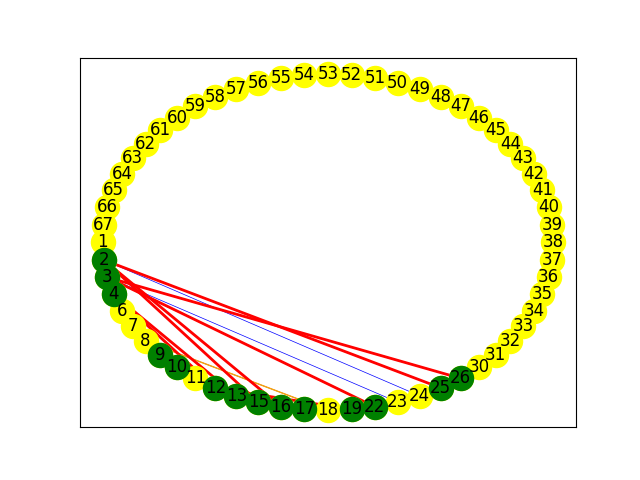
\includegraphics[width=0.7\linewidth]{images/pucp/H_pucp2020_cmp_acm2013_m1_mcs_mix.png}
\caption{IngInform2020 y ACM 2013 MCS modelo 1}
\label{fig:c5p2modelo1}


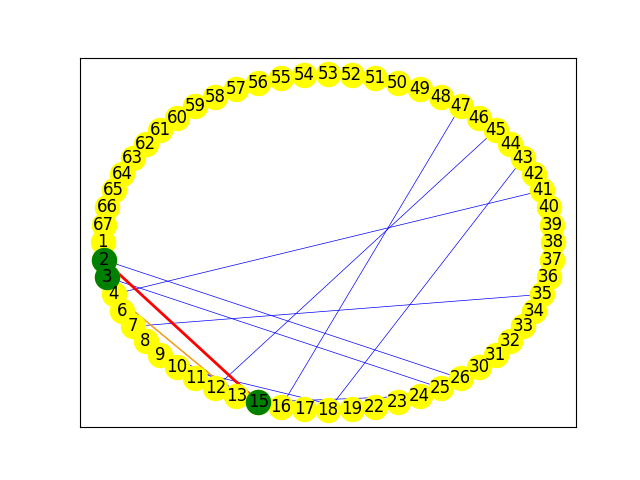
\includegraphics[width=0.7\linewidth]{images/pucp/H_pucp2020_cmp_acm2013_m2_mcs_mix.png}
\caption{IngInform2020 y ACM 2013 MCS modelo 2}
\label{fig:c5p2modelo2}

\end{figure}


\begin{table}[H]
\centering
\caption{Tabulación de datos sobre comparaciones}
\begin{tabular}[t]{|l|l|l|l|l|l|}
\hline
5&model1&26&20&60&20\\
\hline
5&model2&26&20&60&17\\
\hline
\end{tabular}
\label{tab:tabcomparaciones_C5}
\end{table}


\begin{table}[H]
\centering
\caption{MCS}
\begin{tabular}[t]{lccccc}
\hline
Caso & Modelo & MCSsubgrado & similaridad & nodos & enlaces \\
5 & $modelo_1$ & 0.766666666666666 & $z=0.2333333333$ & 18 & 16\\
5 & $modelo_2$ & 0.95 & $z=0.05$ & 5 & 3\\
\hline
\end{tabular}
\label{tab:tabcomparaciones_C5}
\end{table}

\begin{table}[H]
\centering
\caption{Tabla de resultados de proporcionalidad}
\begin{tabular}[t]{lccccccccc}
\hline
Caso & Modelo & nodosCom & enlacesCom & proporcionG &proporcionH \\
5 & $Modelo_1$ & 18 & 16 & $t_1=0.6923076923$ & $t_2=0.3$\\
5 & $Modelo_2$ & 5 & 3 & $t_1=0.1923076923$ & $t_2=0.08333333333$\\
\hline
\end{tabular}
\label{tab:tabresultados2_C5}
\end{table}

\begin{table}[H]
\centering
\caption{Tabla de Hipotesis vs Resultados }
\begin{tabular}[t]{lccccc}
\hline
Hipotesis & Caso & modelo & Similaridad & ProporcionG & ProporcionH\\
P2 & 5 & modelo1 &$z>0.02$&$t_1>0.1$&$t_2>0.1$\\
P2 & 5 & modelo1 &$z<0.02$&$t_1>0.1$&$t_2<0.1$\\
\hline
\end{tabular}
\label{tab:hipotesis_C5}
\end{table}


\clearpage


\subsection{Caso 6 Hipotesis Secundaria 1}

A continuación se muestran las representaciones gráficas y los resultados del $Caso_6$ de la comparación entre un plan de estudio de ingeniería de sistemas(UNI) y una guía internacional ACM 68. En la comparación del modelo 1, se representa con la figura \ref{fig:c6p1modelo1} con grafos y enlaces del modelo ACM y en la figura \ref{fig:c6p1modelo2} que representa cada grafo con sus respectivos enlaces. 

\begin{figure}[H]
\centering
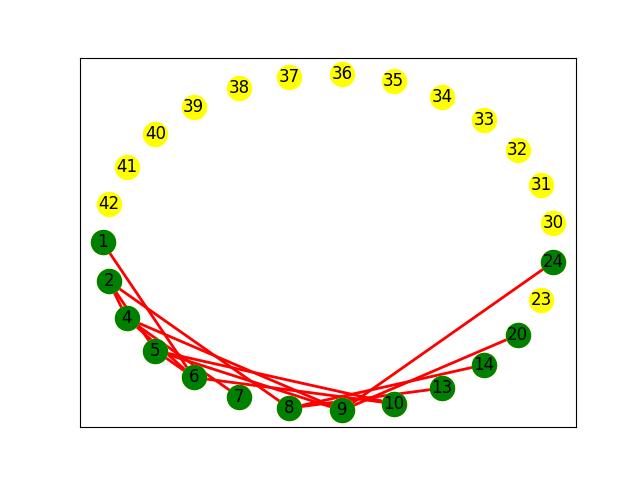
\includegraphics[width=0.7\linewidth]{images/sisuni2018/H_sisuni2018_cmp_acm68_m1_mcs_mix.png}
\caption{IngSistemas2018 y ACM 68 MCS modelo 1}
\label{fig:c6p1modelo1}


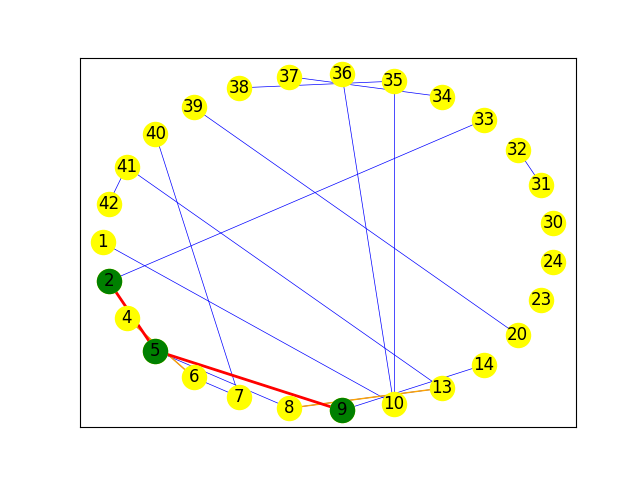
\includegraphics[width=0.7\linewidth]{images/sisuni2018/H_sisuni2018_cmp_acm68_m2_mcs_mix.png}
\caption{IngSistemas2018 y ACM 68 MCS modelo 2}
\label{fig:c6p1modelo2}

\end{figure}


\begin{table}[H]
\centering
\caption{Tabulación de datos sobre comparaciones}
\begin{tabular}[t]{|l|l|l|l|l|l|}
\hline
6&model1&30&39&27&15\\
\hline
6&model2&30&39&27&18\\
\hline
\end{tabular}
\label{tab:tabcomparaciones_C6}
\end{table}


\begin{table}[H]
\centering
\caption{MCS}
\begin{tabular}[t]{lccccc}
\hline
Caso & Modelo & MCSsubgrado & similaridad & nodos & enlaces \\
6 & $modelo_1$ & 0.566666666666667 & $z=0.4333333333$ & 13 & 15\\
6 & $modelo_2$ & 0.9 & $z=0.1$ & 3 & 2\\
\hline
\end{tabular}
\label{tab:tabcomparaciones_C6}
\end{table}

\begin{table}[H]
\centering
\caption{Tabla de resultados de proporcionalidad}
\begin{tabular}[t]{lccccccccc}
\hline
Caso & Modelo & nodosCom & enlacesCom & proporcionG &proporcionH \\
6 & $Modelo_1$ & 13 & 15 & $t_1=0.43$ & $t_2=0.3$\\
6 & $Modelo_2$ & 7 & 4 & $t_1=0.1$ & $t_2=0.08333333333$\\
\hline
\end{tabular}
\label{tab:tabresultados2_C5_P1}
\end{table}

\begin{table}[H]
\centering
\caption{Tabla de Hipotesis vs Resultados }
\begin{tabular}[t]{lccccc}
\hline
Hipotesis & Caso & modelo & Similaridad & ProporcionG & ProporcionH\\
P1 & 6 & modelo1 &$z>0.02$&$t_1>0.1$&$t_2>0.1$\\
P1 & 6 & modelo2 &$z<0.02$&$t_1<0.1$&$t_2<0.1$\\
\hline
\end{tabular}
\label{tab:hipotesis_C6}
\end{table}



\section{Resultados}

Como podemos observar no en todos los casos se logra obtener una similaridad mínima es decir cuando $z > 0.2 $ lo que invalida el caso de la hipótesis considerada en el estudio. El uso o no de las relaciones originales en la equivalencia de cursos. Es decir cuando usamos las relaciones originales de las curriculas internacionales se encuentra más casos de similaridad, pero también se encuentran casos que teniendo las relaciones del $Modelo_2$ se da un grado de similaridad. Esto es importante subrayar pues el modelamiento y la comparación nos puede dar pistas sobre que áreas y que cursos servirán como elementos para una incorporación o adaptación a perfiles de una curricula o guía internacional sin que eso afecte la estructura orgánica de la propuesta educativa.

En el caso del indicador $t > 0.1$ podemos observar el cumplimiento de los casos de proporcionalidad con mayor incidencia en el $Modelo_1$ eso nos da una pista que en algunos casos las relaciones de dependencia de las guías internacionales pueden acercar más la adopción de los referentes en contraste a que las instituciones usan sus propios esquemas de dependencia entre cursos, es decir no solo es necesario incorporar cursos y áreas de conocimiento sino también observar las dependencias entre estos cursos o contenidos. 


\clearpage

\section{Conclusiones}

\begin{enumerate}
	\item El modelamiento en grafos para la información de planes de estudio como de guias internacionales y habilitar la opción de comparación con indicadores numéricos es una herramienta novedosa para abordar el proceso de innovación curricular de las instituciones. 
	\item Más allá de las diferencias estructurales o históricas de las escuelas peruanas, utilizando herramientas como las propuestas en el presente estudio una institución puede observar el cambio en el tiempo y la adaptación a los distintos enfoques que va teniendo del diseño curricular. Además que puede observar si esa orientación refleja algún perfil o contenido central. El alcance de esta investigación no ha abordado la comparación en concreto de niveles de profundidad o tipos de orientación de los cursos, dado que eso implicaría un nivel más elaborado de comparaciones. Pero si se plantea el método y los mecanismos que pueden permitir ese nivel de evaluación de esos casos.
	\item El plantear comparaciones entre planes de estudio de la diversidad de oferta educativa así como encontrar similitudes con guías internacionales apoya la inclusión de los referentes internacionales así como puntos de partida para las instituciones.
	\item La inclusión de un modelo de referente internacional como el ACM68 y compararlo con al menos un plan de estudio antiguo de una universidad nos sirve para encontrar pistas de la influencia de la computación internacional en décadas pasadas y en parte también dar pistas que los planes de estudio pueden seguir la línea de profesiones de informática internacional así lleven nombres de profesiones de ingeniería.

\end{enumerate}

\newpage

\section{Trabajos futuros}

El mundo de la educación en informática es cambiante como la disciplina misma, mientras se le observa se va adaptando y cambiando en el tiempo. Sin embargo lo que menos cambia es la institucionalidad y eso se refleja tanto en los diseños orgánicos de las instituciones educativas como de los planes de oferta educativa, las personas y los elementos culturales. Innovar en estos sistemas sociales es un verdadero desafío que solo tiene sentido con el impulso de cada organización. Este estudio se presenta como una oportunidad para contribuir con herramientas de análisis cuantitativo en el estudio del desarrollo de los cambios y de la arquitectura interna de las relaciones de los contenidos y cursos de los programas educativos. Es un factor que no deberíamos ignorar como un elemento que nos permita contribuir en el desarrollo de los diseños curriculares y observar los movimientos y relaciones que puedan existir en los programas académicos.

Como trabajos futuros quedan poder hacer comparaciones a nivel de competencias de los planes de estudio y sus correspondientes guías internacionales o pares educativos. También poder hacer comparaciones a nivel de propiedades de los grafos, como por ejemplo el nivel de orientación teórico práctico de una grafo que corresponda a una unidad de conocimiento o curso. Poder realizar análisis de concentraciones o de agrupamientos de áreas también puede mejorar la toma de decisiones en la planificación educativa y vincular eso a otras necesidades económicas como industriales.

En cierta forma el modelamiento de los grafos y sus relaciones requiere juicio de análisis y por ende corre riesgo de introducir errores de interpretación, sin embargo esto puede reducirse conforme se puedan lograr consensos e interpretaciones por contenidos de los cursos. Es decir aplicando técnicas estadísticas y umbrales de aproximación en los contenidos de los cursos se podría lograr niveles de equivalencias entre nodos luego de las relaciones y poder ejecutar comparaciones más cercanas o automatizadas, introducir una capacidad de generalidad y escalamiento del proceso. 

Finalmente esta línea de investigación abre posibilidades para generar mejoras en la educación universitaria desde la comunidad académica de la informática en nuestras universidades.